% This LaTeX was auto-generated from MATLAB code.
% To make changes, update the MATLAB code and export to LaTeX again.

\documentclass{article}

\usepackage[utf8]{inputenc}
\usepackage[T1]{fontenc}
\usepackage{lmodern}
\usepackage{graphicx}
\usepackage{color}
\usepackage{hyperref}
\usepackage{amsmath}
\usepackage{amsfonts}
\usepackage{epstopdf}
\usepackage[table]{xcolor}
\usepackage{matlab}

\sloppy
\epstopdfsetup{outdir=./}
\graphicspath{ {./assignment_5_code_images/} }

\begin{document}

\begin{matlabcode}
warning('off','all')
\end{matlabcode}


\begin{par}
\begin{flushleft}
Question: 2.a)
\end{flushleft}
\end{par}

\begin{matlabcode}
b1 = 3; b2 = 2.1; b3 = 0.6;
G = tf([b1,b2,b3],[1],1,"Variable","z^-1");

N = 2046; p = 3;
uk = idinput(2046,'PRBS', [0 0.2], [-1 1]);
ykstar = lsim(G,uk);
    
ek = randn([2046,1]);
noise_var = var(ykstar)/10;
yk = ykstar + ek*sqrt(noise_var);

\end{matlabcode}

\begin{par}
\begin{flushleft}
Question: 2.b)
\end{flushleft}
\end{par}

\begin{matlabcode}
phi = [];
for k = 4:2047
    phi = [phi; [uk(k-1) uk(k-2) uk(k-3)]];
end

theta_hat = pinv(phi)*yk(3:end)
\end{matlabcode}
\begin{matlaboutput}
theta_hat = 3x1    
    3.0379
    2.0247
    0.6465

\end{matlaboutput}


\begin{par}
\begin{flushleft}
Question: 2.c)
\end{flushleft}
\end{par}

\begin{matlabcode}
y_hat = phi*theta_hat;
residual = yk(3:end) - y_hat;

noise_var_hat = sum(residual.^2)/ (N-p)
\end{matlabcode}
\begin{matlaboutput}
noise_var_hat = 2.7803
\end{matlaboutput}
\begin{matlabcode}
cov_theta_hat = inv(transpose(phi)*phi) * noise_var_hat
\end{matlabcode}
\begin{matlaboutput}
cov_theta_hat = 3x3    
    0.0038   -0.0034    0.0004
   -0.0034    0.0068   -0.0034
    0.0004   -0.0034    0.0038

\end{matlaboutput}
\begin{matlabcode}

for i = 1:3
    u = theta_hat(i) + 1.96*sqrt(cov_theta_hat(i,i));
    l = theta_hat(i) - 1.96*sqrt(cov_theta_hat(i,i));
    fprintf('Confidence Interval of theta%d: (%f,%f) \n',i,u,l)
end
\end{matlabcode}
\begin{matlaboutput}
Confidence Interval of theta1: (3.158944,2.916799) 
Confidence Interval of theta2: (2.186292,1.863092) 
Confidence Interval of theta3: (0.767792,0.525121) 
\end{matlaboutput}


\begin{par}
\begin{flushleft}
Question: 2.d) and 2.f)
\end{flushleft}
\end{par}

\begin{matlabcode}
theta_hat = [];
b = [b1 b2 b3];
theta_count = [0 0 0];

for i = 1:100
    uk = idinput(2046,'PRBS', [0 0.2], [-1 1]);
    ykstar = lsim(G,uk);
        
    ek = randn([2046,1]);
    noise_var = var(ykstar)/10;
    yk = ykstar + ek*sqrt(noise_var);
       
    dataset = iddata(yk,uk,1);
    [Ztrain,Tr] = detrend(dataset,0);
    
    phi = [];
    for k = 4:2047
        phi = [phi; [uk(k-1) uk(k-2) uk(k-3)]];
    end
    
    theta = pinv(phi)*yk(3:end);
    theta_hat = [theta_hat theta];
    cov_theta_hat = inv(transpose(phi)*phi) * noise_var;
    
    % Confidence 
    for i = 1:3
        u = theta(i) + 1.96*sqrt(cov_theta_hat(i,i));
        l = theta(i) - 1.96*sqrt(cov_theta_hat(i,i));
        
        if((b(i) > l) && (b(i) < u))
            theta_count(i) = theta_count(i) + 1;
        end
    end
end

mean(transpose(theta_hat))
\end{matlabcode}
\begin{matlaboutput}
ans = 1x3    
    3.0016    2.1046    0.5958

\end{matlaboutput}
\begin{matlabcode}
cov(transpose(theta_hat))
\end{matlabcode}
\begin{matlaboutput}
ans = 3x3    
    0.0044   -0.0049    0.0009
   -0.0049    0.0084   -0.0033
    0.0009   -0.0033    0.0031

\end{matlaboutput}
\begin{matlabcode}
theta_count
\end{matlabcode}
\begin{matlaboutput}
theta_count = 1x3    
    91    91    96

\end{matlaboutput}

\begin{par}
\begin{flushleft}
Question: 2.e)
\end{flushleft}
\end{par}

\begin{matlabcode}
% Theoretical co-variance
cov_theta_hat = inv(transpose(phi)*phi) * noise_var
\end{matlabcode}
\begin{matlaboutput}
cov_theta_hat = 3x3    
    0.0038   -0.0034    0.0004
   -0.0034    0.0069   -0.0034
    0.0004   -0.0034    0.0039

\end{matlaboutput}

\begin{par}
\begin{flushleft}
Question: 2.g)
\end{flushleft}
\end{par}

\begin{matlabcode}
set(gcf,'position',[10,10,1500,300])

subplot(1,3,1);
histogram(theta_hat(1,:));
title('b1 hat');

subplot(1,3,2);
histogram(theta_hat(2,:));
title('b2 hat');

subplot(1,3,3);
histogram(theta_hat(3,:));
title('b3 hat');
\end{matlabcode}
\begin{center}
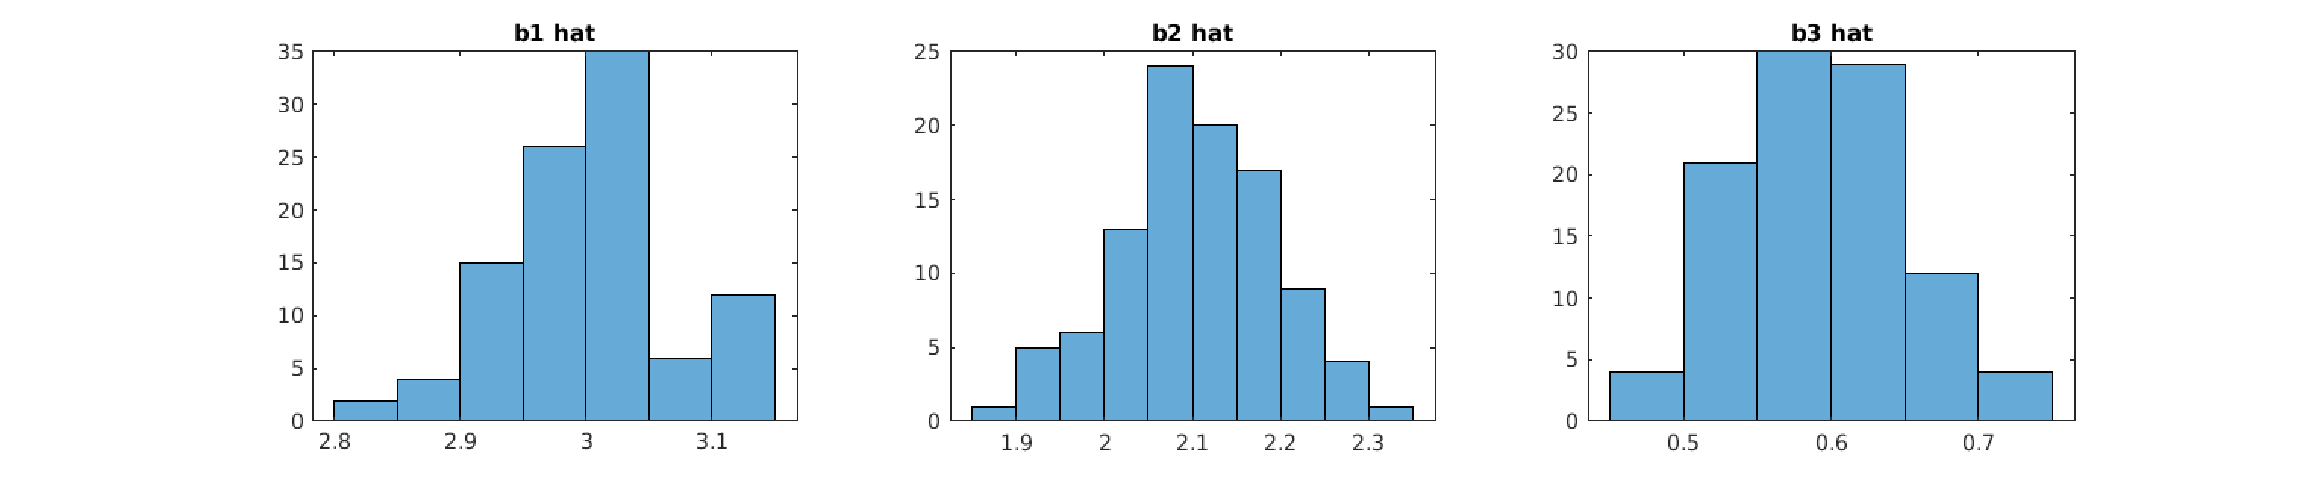
\includegraphics[width=\maxwidth{128.44957350727546em}]{figure_0.eps}
\end{center}


\begin{par}
\begin{flushleft}
Question: 3.a)
\end{flushleft}
\end{par}

\begin{matlabcode}
mod_p = idpoly (1, [0,0,0,2,0.6], 1, [1 -0.5], [1,-1.2,0.32],'Noisevariance', 1,'Ts',1)
\end{matlabcode}
\begin{matlaboutput}
mod_p =
Discrete-time Polynomial model: y(t) = [B(z)/F(z)]u(t) + [1/D(z)]e(t)
  B(z) = 2 z^-3 + 0.6 z^-4                                           
                                                                     
  D(z) = 1 - 0.5 z^-1                                                
                                                                     
  F(z) = 1 - 1.2 z^-1 + 0.32 z^-2                                    
                                                                     
Sample time: 1 seconds
  
Parameterization:
   Polynomial orders:   nb=2   nd=1   nf=2   nk=3
   Number of free coefficients: 5
   Use "polydata", "getpvec", "getcov" for parameters and their uncertainties.

Status:                                                         
Created by direct construction or transformation. Not estimated.
\end{matlaboutput}
\begin{matlabcode}
uk = idinput(1530,'PRBS', [0 0.15], [-1 1]);

% Calculate yk_star:
yk_star = sim(mod_p ,uk);

% Calculate variance of e[k] such that var(yk_star)/var(v[k]) = 10
mod_p.Noisevariance = var(yk_star) * 0.075;
yk = sim(mod_p ,uk , simOptions ('AddNoise',true));

\end{matlabcode}

\begin{par}
\begin{flushleft}
Question: 3.b)
\end{flushleft}
\end{par}

\begin{matlabcode}
% Train-Test split:
dataset = iddata(yk ,uk ,1);
datatrain = dataset (1:1000); datatest = dataset (1001:end);
[Ztrain ,Tr] = detrend(datatrain, 0);
Ztest = detrend(datatest, Tr);

% 99 % significance levels
clim = 2.58/sqrt(length(Ztrain.y));
\end{matlabcode}


\begin{par}
\begin{flushleft}
Question: 3.c)
\end{flushleft}
\end{par}

\begin{matlabcode}
% ARX model:
mod_arx = arx(Ztrain, [2 3 3]);
present(mod_arx)
\end{matlabcode}
\begin{matlaboutput}
                                                                                   
mod_arx =                                                                          
Discrete-time ARX model: A(z)y(t) = B(z)u(t) + e(t)                                
  A(z) = 1 - 0.5564 (+/- 0.03066) z^-1 - 0.1965 (+/- 0.02641) z^-2                 
                                                                                   
  B(z) = 1.58 (+/- 0.2327) z^-3 + 2.275 (+/- 0.3176) z^-4 + 1.261 (+/- 0.2728) z^-5
                                                                                   
Sample time: 1 seconds                                                             
                                                                                   
Parameterization:                                                                  
   Polynomial orders:   na=2   nb=3   nk=3                                         
   Number of free coefficients: 5                                                  
   Use "polydata", "getpvec", "getcov" for parameters and their uncertainties.     
                                                                                   
Status:                                                                            
Estimated using ARX on time domain data "Ztrain".                                  
Fit to estimation data: 73.63% (prediction focus)                                  
FPE: 16.01, MSE: 15.75                                                             
More information in model's "Report" property.                                     
\end{matlaboutput}
\begin{matlabcode}
yhat_arx = predict(mod_arx, Ztrain );      % Predictions on training data
err_arx = pe(mod_arx , Ztrain );           % Compute one-step ahead prediction errors

% Residual analysis:
cross_corr_arx = xcov(err_arx.y, Ztrain.u, 100,'coeff');
acf_arx = xcov(err_arx.y,50,'coeff');

% Plot
figure;set(gcf,'position',[10,10,1000,900]);

subplot(311); stem( -100:100 , cross_corr_arx ); hold on
plot([ -100 100] ,[1 1]* clim ,'r--' ,[-100 100], [ -1 -1]*clim ,'g--')
title('Correlation between residuals and inputs (ARX Model)')

subplot(312); stem((0:50) ,acf_arx (51:end)); hold on
plot([0 50] ,[1 1]* clim ,'r--' ,[0 50] ,[ -1 -1]*clim ,'g--')
title('Auto-correlation funtion of residuals (ARX Model)')

subplot(313)
test_prediction = predict(mod_arx, Ztest);
plot(test_prediction.y, Ztest.y, 'x', Ztest.y, Ztest.y, 'r-');
title('Predictions on test data')
\end{matlabcode}
\begin{center}
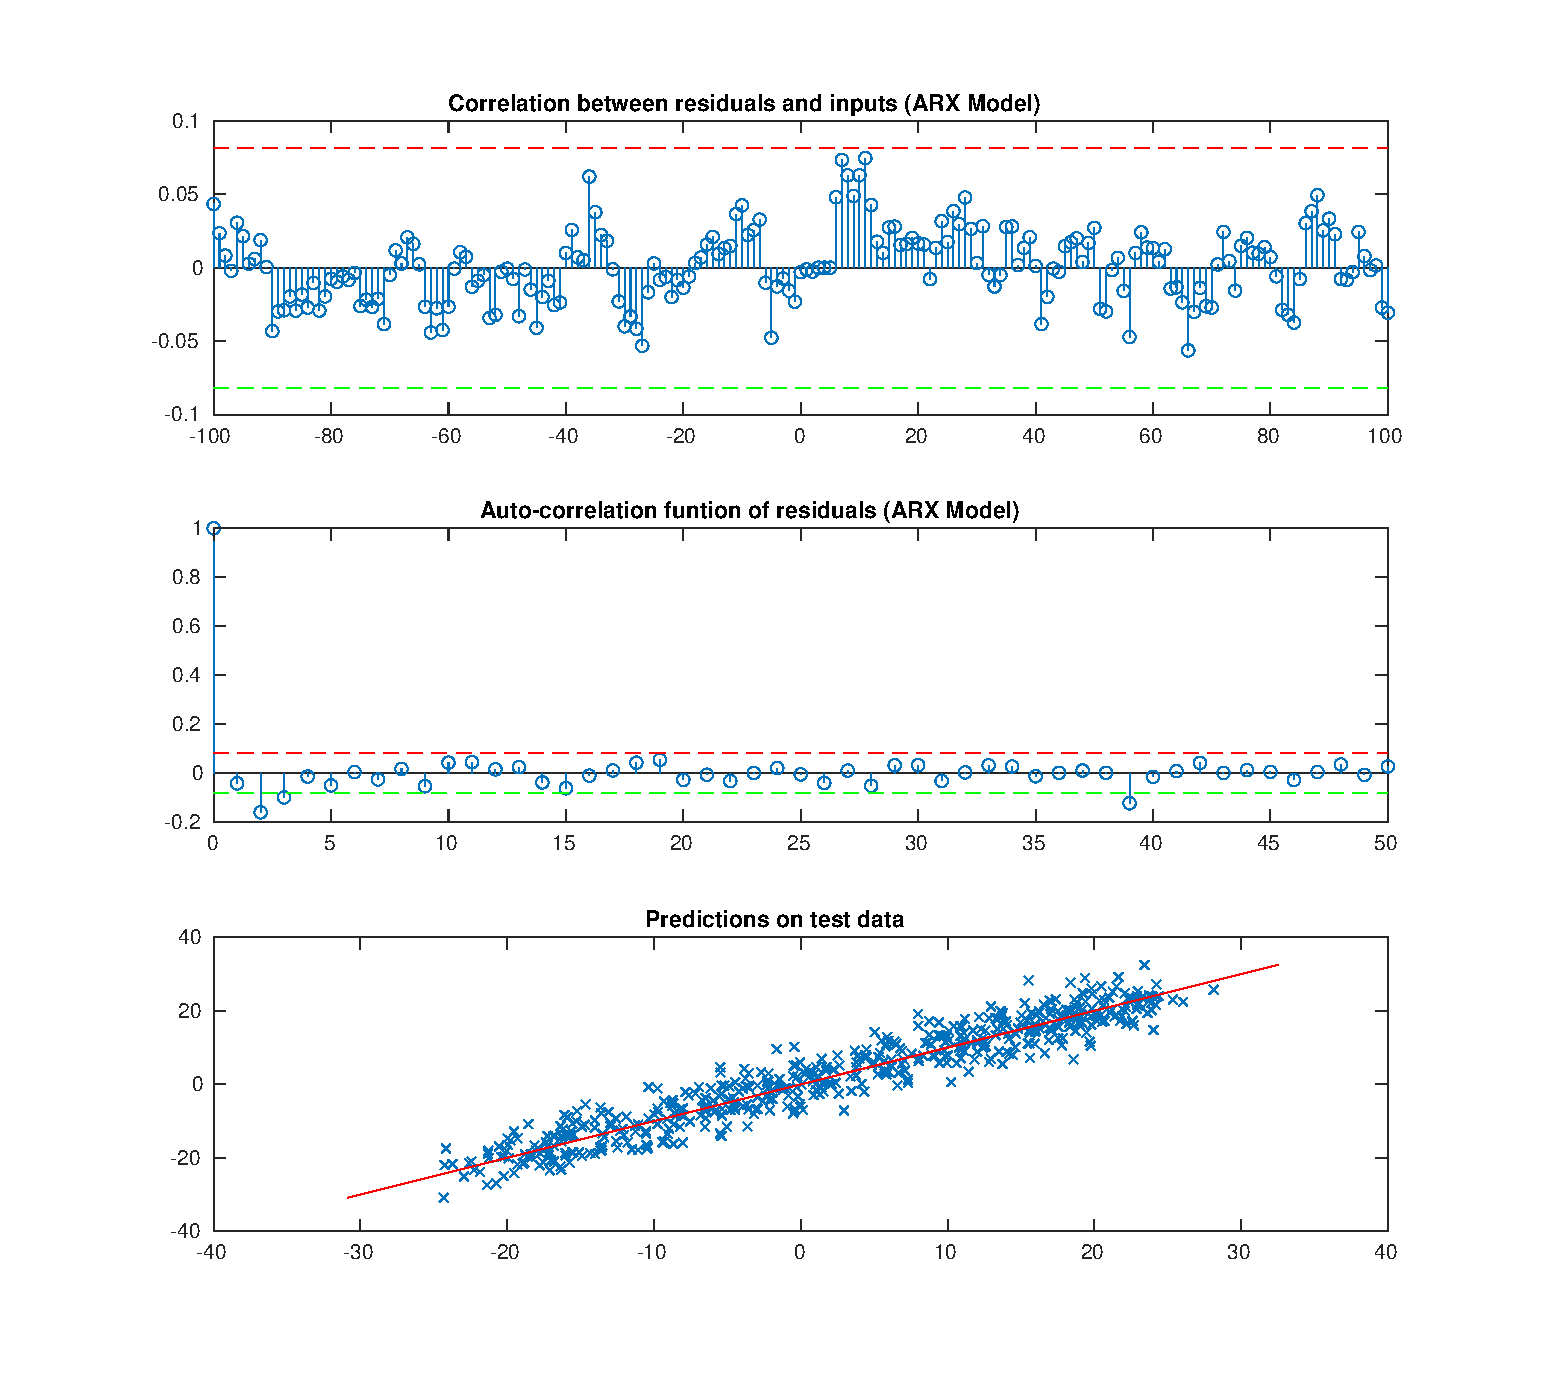
\includegraphics[width=\maxwidth{89.20109271338573em}]{figure_1.eps}
\end{center}
\begin{matlabcode}
R_squared = 1 - norm(Ztest.y - test_prediction.y)/norm(Ztest.y - mean(Ztest.y))
\end{matlabcode}
\begin{matlaboutput}
R_squared = 0.7071
\end{matlaboutput}


\begin{matlabcode}
% OE model:
mod_oe = oe(Ztrain ,[2 1 3]);
present(mod_oe)
\end{matlabcode}
\begin{matlaboutput}
                                                                              
mod_oe =                                                                      
Discrete-time OE model: y(t) = [B(z)/F(z)]u(t) + e(t)                         
  B(z) = 1.255 (+/- 0.2531) z^-3 + 2.567 (+/- 0.294) z^-4                     
                                                                              
  F(z) = 1 - 0.828 (+/- 0.005994) z^-1                                        
                                                                              
Sample time: 1 seconds                                                        
                                                                              
Parameterization:                                                             
   Polynomial orders:   nb=2   nf=1   nk=3                                    
   Number of free coefficients: 3                                             
   Use "polydata", "getpvec", "getcov" for parameters and their uncertainties.
                                                                              
Status:                                                                       
Termination condition: Near (local) minimum, (norm(g) < tol)..                
Number of iterations: 2, Number of function evaluations: 5                    
                                                                              
Estimated using OE on time domain data "Ztrain".                              
Fit to estimation data: 71.07%                                                
FPE: 19.08, MSE: 18.96                                                        
More information in model's "Report" property.                                
\end{matlaboutput}
\begin{matlabcode}
yhat_oe = predict(mod_oe , Ztrain );       % Predictions on training data
err_oe = pe(mod_oe , Ztrain );             % Compute one-step ahead prediction errors

% Residual analysis:
cross_corr_oe = xcov(err_oe.y, Ztrain.u,25,'coeff');
acf_oe = xcov(err_oe.y,20,'coeff');

% Plot
figure;set(gcf,'position',[10,10,1000,900]);

subplot(311); stem( -25:25 , cross_corr_oe ); hold on
plot([ -25 25] ,[1 1]* clim ,'r--' ,[-25 25] ,[ -1 -1]*clim ,'g--')
title('Correlation between residuals and inputs (OE Model)')

subplot(312); stem((0:20) ,acf_oe (21:end)); hold on
plot([0 20] ,[1 1]* clim ,'r--' ,[0 20] ,[ -1 -1]*clim ,'g--')
title('Auto-correlation funtion of residuals (OE Model)')

subplot(313)
test_prediction = predict(mod_oe, Ztest);
plot(test_prediction.y, Ztest.y, 'x', Ztest.y, Ztest.y, 'r-');
title('Predictions on test data')
\end{matlabcode}
\begin{center}
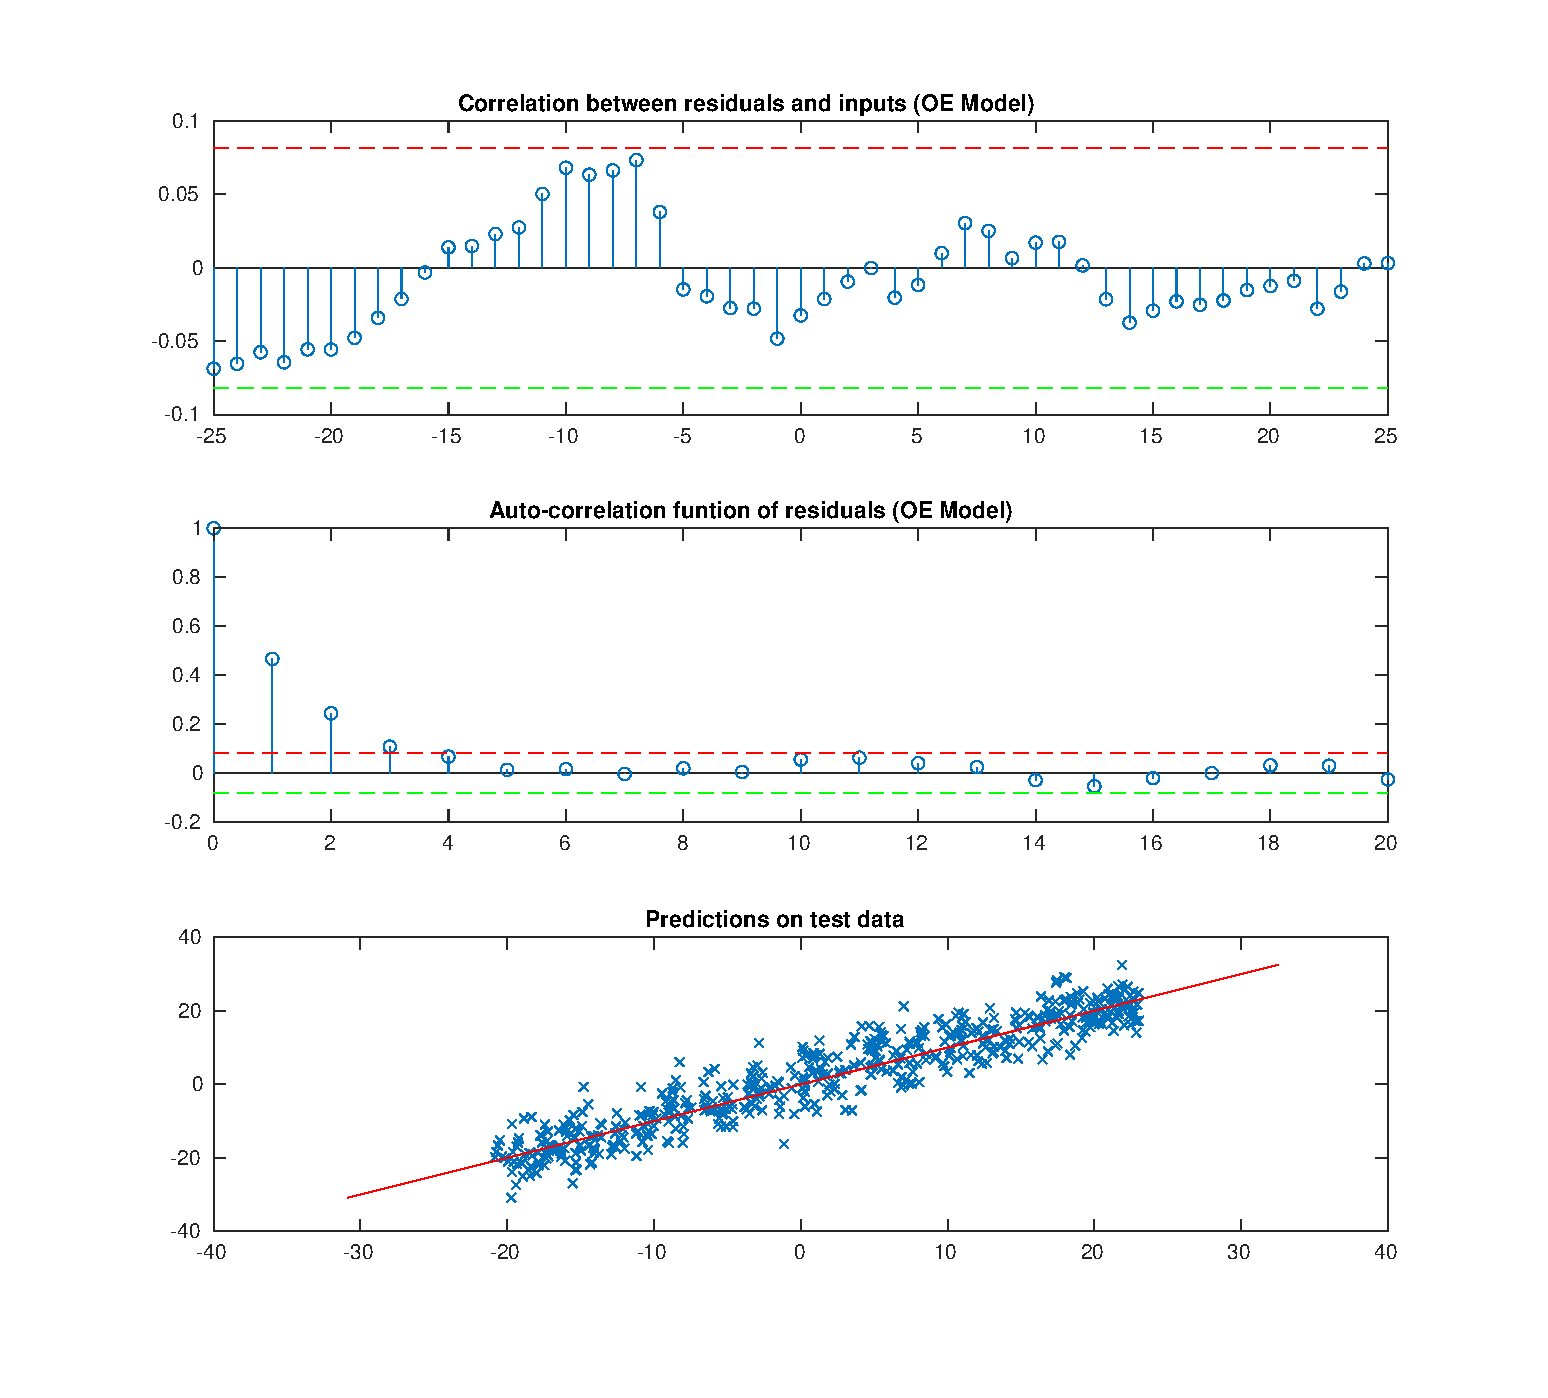
\includegraphics[width=\maxwidth{89.20109271338573em}]{figure_2.eps}
\end{center}
\begin{matlabcode}
R_squared = 1 - norm(Ztest.y - test_prediction.y)/norm(Ztest.y - mean(Ztest.y))
\end{matlabcode}
\begin{matlaboutput}
R_squared = 0.6637
\end{matlaboutput}
\begin{matlabcode}
% BJ model:
mod_bj = bj(Ztrain ,[2 0 1 1 3]);
present(mod_bj)
\end{matlabcode}
\begin{matlaboutput}
                                                                              
mod_bj =                                                                      
Discrete-time Polynomial model: y(t) = [B(z)/F(z)]u(t) + [1/D(z)]e(t)         
  B(z) = 1.478 (+/- 0.2127) z^-3 + 2.294 (+/- 0.2468) z^-4                    
                                                                              
  D(z) = 1 - 0.4707 (+/- 0.02797) z^-1                                        
                                                                              
  F(z) = 1 - 0.8314 (+/- 0.00556) z^-1                                        
                                                                              
Sample time: 1 seconds                                                        
                                                                              
Parameterization:                                                             
   Polynomial orders:   nb=2   nd=1   nf=1   nk=3                             
   Number of free coefficients: 4                                             
   Use "polydata", "getpvec", "getcov" for parameters and their uncertainties.
                                                                              
Status:                                                                       
Termination condition: Near (local) minimum, (norm(g) < tol)..                
Number of iterations: 2, Number of function evaluations: 6                    
                                                                              
Estimated using BJ on time domain data "Ztrain".                              
Fit to estimation data: 74.46% (prediction focus)                             
FPE: 14.9, MSE: 14.78                                                         
More information in model's "Report" property.                                
\end{matlaboutput}
\begin{matlabcode}
yhat_bj = predict(mod_bj, Ztrain );       % Predictions on training data
err_bj = pe(mod_bj, Ztrain );             % Compute one-step ahead prediction errors

% Residual analysis:
cross_corr_bj = xcov(err_bj.y, Ztrain.u,25,'coeff');
acf_bj = xcov(err_bj.y,20,'coeff');

% Plot
figure;set(gcf,'position',[10,10,1000,900]);

subplot(311); stem( -25:25 , cross_corr_bj ); hold on
plot([ -25 25] ,[1 1]* clim ,'r--' ,[-25 25] ,[ -1 -1]*clim ,'g--')
title('Correlation between residuals and inputs (BJ Model)')

subplot(312); stem((0:20) ,acf_bj (21:end)); hold on
plot([0 20] ,[1 1]* clim ,'r--' ,[0 20] ,[ -1 -1]*clim ,'g--')
title('Auto-correlation funtion of residuals (BJ Model)')

subplot(313)
test_prediction = predict(mod_bj, Ztest);
plot(test_prediction.y, Ztest.y, 'x', Ztest.y, Ztest.y, 'r-');
title('Predictions on test data')
\end{matlabcode}
\begin{center}
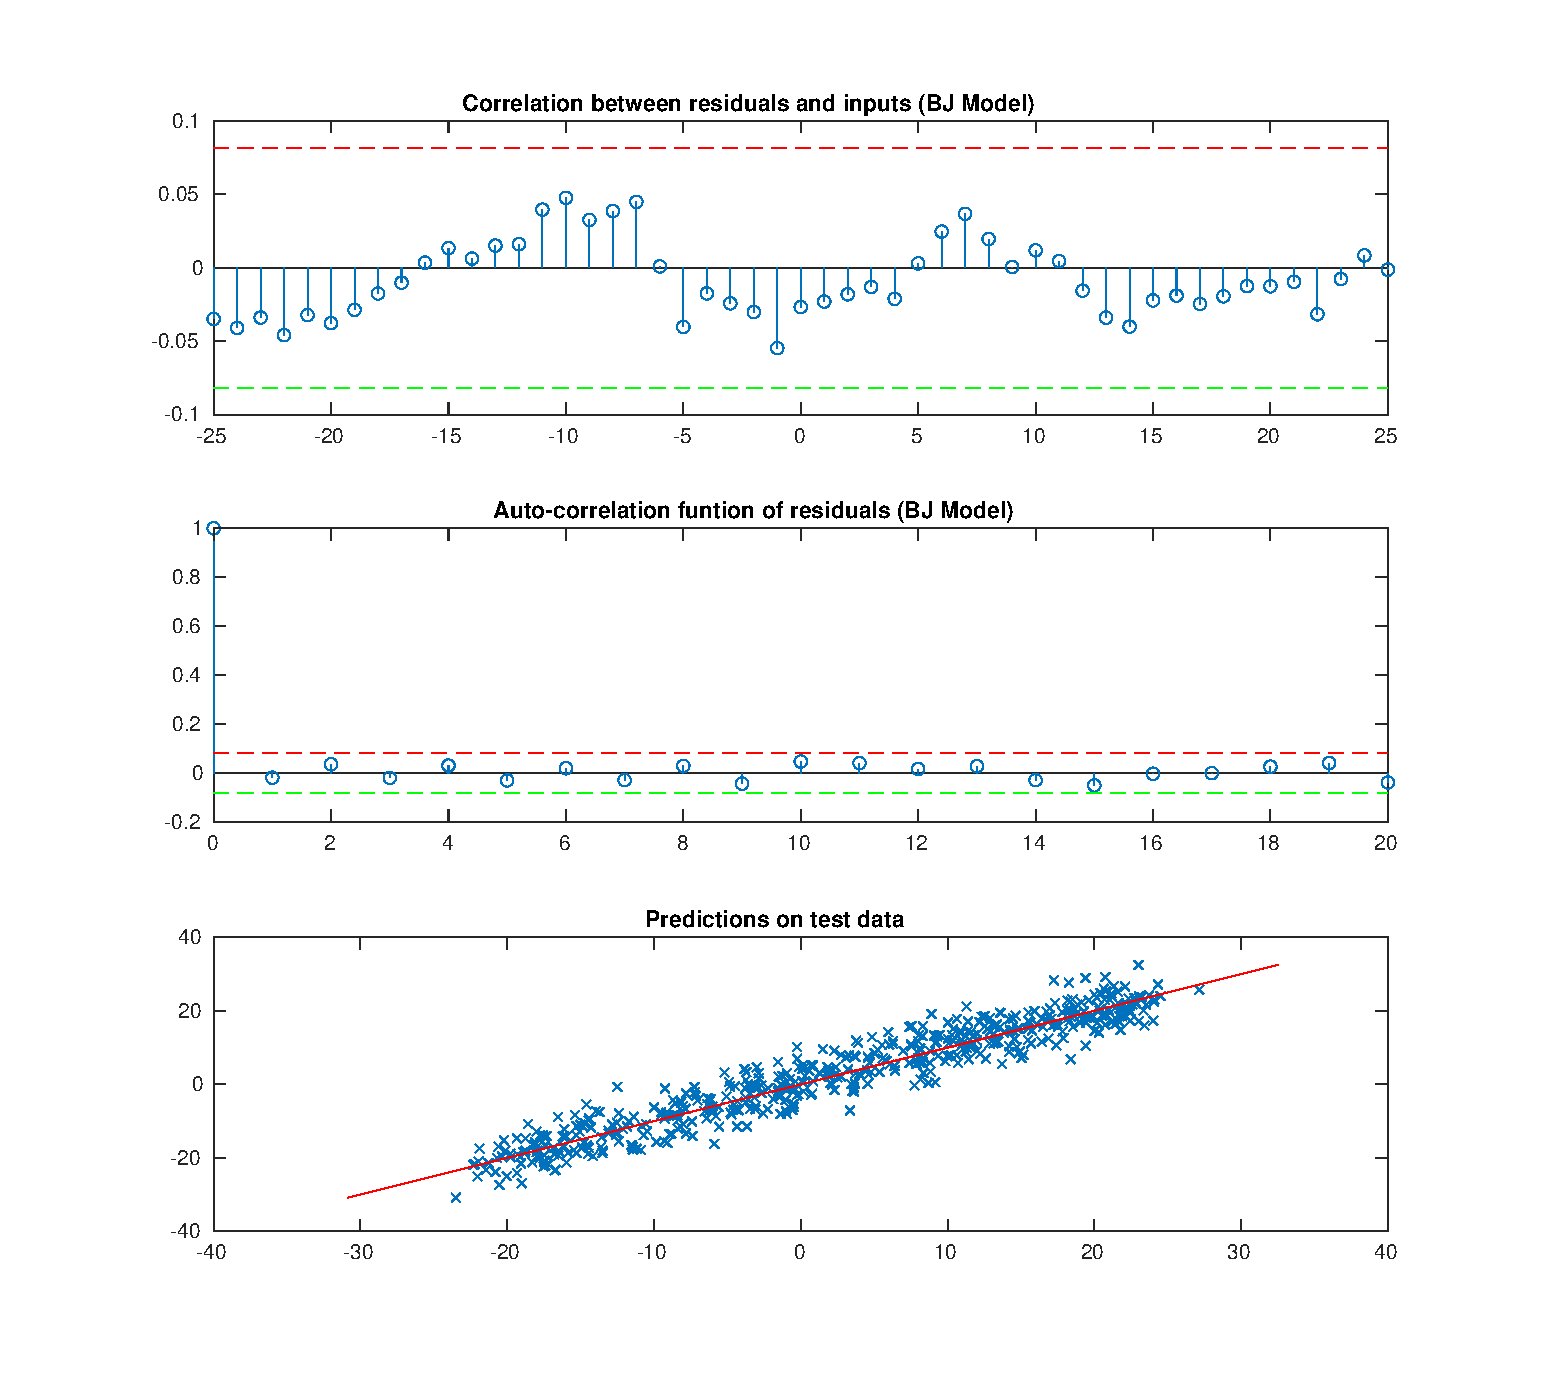
\includegraphics[width=\maxwidth{89.20109271338573em}]{figure_3.eps}
\end{center}
\begin{matlabcode}
R_squared = 1 - norm(Ztest.y - test_prediction.y)/norm(Ztest.y - mean(Ztest.y))
\end{matlabcode}
\begin{matlaboutput}
R_squared = 0.7147
\end{matlaboutput}

\begin{par}
\begin{flushleft}
Question: 4.a)
\end{flushleft}
\end{par}

\begin{matlabcode}
iodata= load("a5_inoutdata.mat");
% Check for Integrating effects:
figure;set(gcf,'position',[10,10,1000,600]);

subplot(2,1,1)
plot(iodata.yk)

subplot(2,1,2)
plot(iodata.yk(2:end) - iodata.yk(1:end-1))
\end{matlabcode}
\begin{center}
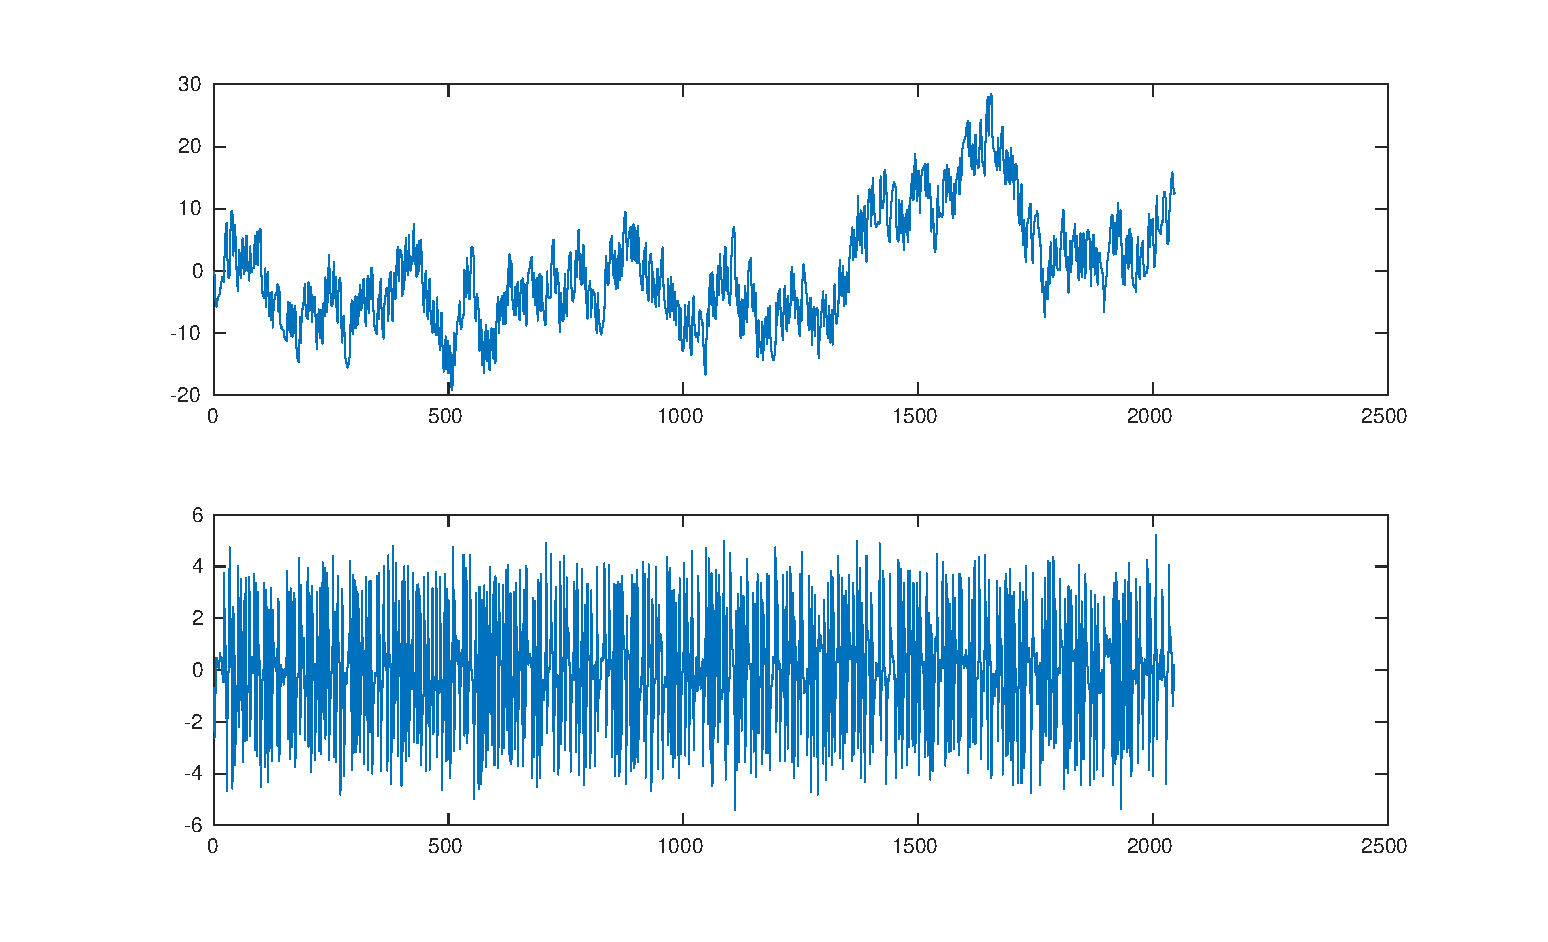
\includegraphics[width=\maxwidth{100.35122930255896em}]{figure_4.eps}
\end{center}
\begin{matlabcode}
% Estimating delay using impulse responses
irestoptions = impulseestOptions;
irestoptions.Advanced.AROrder = 0;
mod_ir = impulseest(iddata(iodata.yk, iodata.uk, 1),irestoptions);

% Plot the IR coefficients
[ircoeff,kvec,q,ir_sd] = impulse(mod_ir,70);
figure;
stem(kvec,ircoeff,'Markerfacecolor','blue');
\end{matlabcode}
\begin{center}
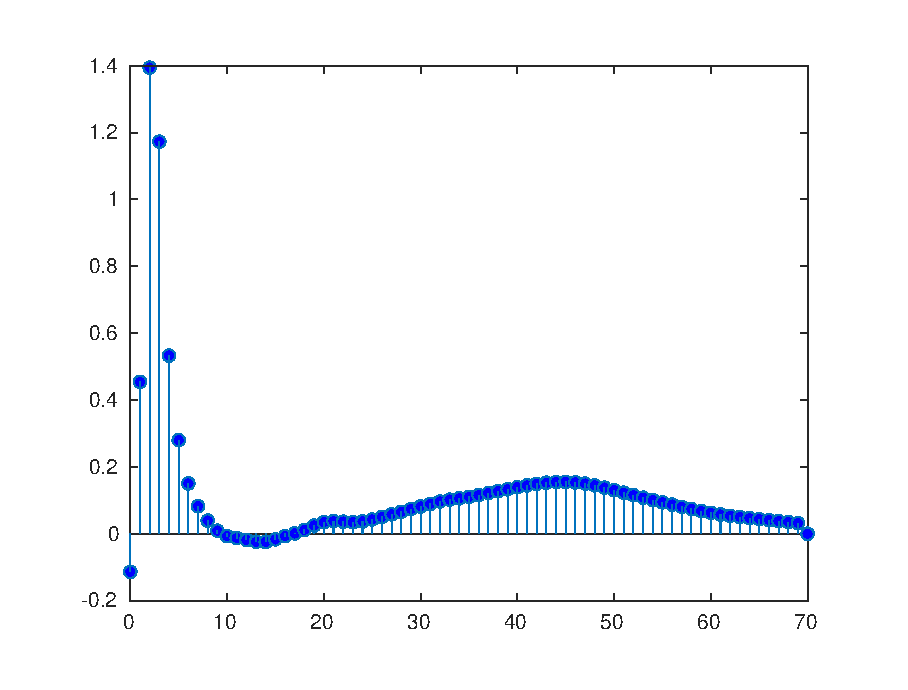
\includegraphics[width=\maxwidth{57.90265930757652em}]{figure_5.eps}
\end{center}



\vspace{1em}
\begin{par}
\begin{center}
Removing integrating effects:
\end{center}
\end{par}

\begin{matlabcode}
% Train-Test split: (removing integrating effects)
dataset = iddata(iodata.yk(2:end) - iodata.yk(1:end-1) ,iodata.uk(2:end) - iodata.uk(1:end-1) ,1);
datatrain = dataset (1:1500); datatest = dataset (1501:end);
[Ztrain ,Tr] = detrend(datatrain, 0);
Ztest = detrend(datatest, Tr);

% 99 % significance levels
clim = 2.58/sqrt(length(Ztrain.y));
\end{matlabcode}


\vspace{1em}
\begin{par}
\begin{center}
OE model: (white-noise assumption)
\end{center}
\end{par}

\begin{matlabcode}
% OE model:
mod_oe = oe(Ztrain ,[1 1 2]);
present(mod_oe);
\end{matlabcode}
\begin{matlaboutput}
                                                                              
mod_oe =                                                                      
Discrete-time OE model: y(t) = [B(z)/F(z)]u(t) + e(t)                         
  B(z) = 2.008 (+/- 0.01363) z^-2                                             
                                                                              
  F(z) = 1 - 0.5143 (+/- 0.007191) z^-1                                       
                                                                              
Sample time: 1 seconds                                                        
                                                                              
Parameterization:                                                             
   Polynomial orders:   nb=1   nf=1   nk=2                                    
   Number of free coefficients: 2                                             
   Use "polydata", "getpvec", "getcov" for parameters and their uncertainties.
                                                                              
Status:                                                                       
Termination condition: Near (local) minimum, (norm(g) < tol)..                
Number of iterations: 1, Number of function evaluations: 3                    
                                                                              
Estimated using OE on time domain data "Ztrain".                              
Fit to estimation data: 75.26%                                                
FPE: 0.2697, MSE: 0.269                                                       
More information in model's "Report" property.                                
\end{matlaboutput}
\begin{matlabcode}
yhat_oe = predict(mod_oe , Ztrain );       % Predictions on training data
err_oe = pe(mod_oe , Ztrain );             % Compute one-step ahead prediction errors

% Residual analysis:
cross_corr_oe = xcov(err_oe.y, Ztrain.u,25,'coeff');
acf_oe = xcov(err_oe.y,20,'coeff');

% Plot
figure;set(gcf,'position',[10,10,1000,600]);

subplot(211); stem( -25:25 , cross_corr_oe ); hold on
plot([ -25 25] ,[1 1]* clim ,'r--' ,[-25 25] ,[ -1 -1]*clim ,'g--')
title('Correlation between residuals and inputs (OE Model)')
ylim([-0.1 0.1])
subplot(212); stem((0:20) ,acf_oe (21:end)); hold on
plot([0 20] ,[1 1]* clim ,'r--' ,[0 20] ,[ -1 -1]*clim ,'g--')
title('Auto-correlation funtion of residuals (OE Model)')
\end{matlabcode}
\begin{center}
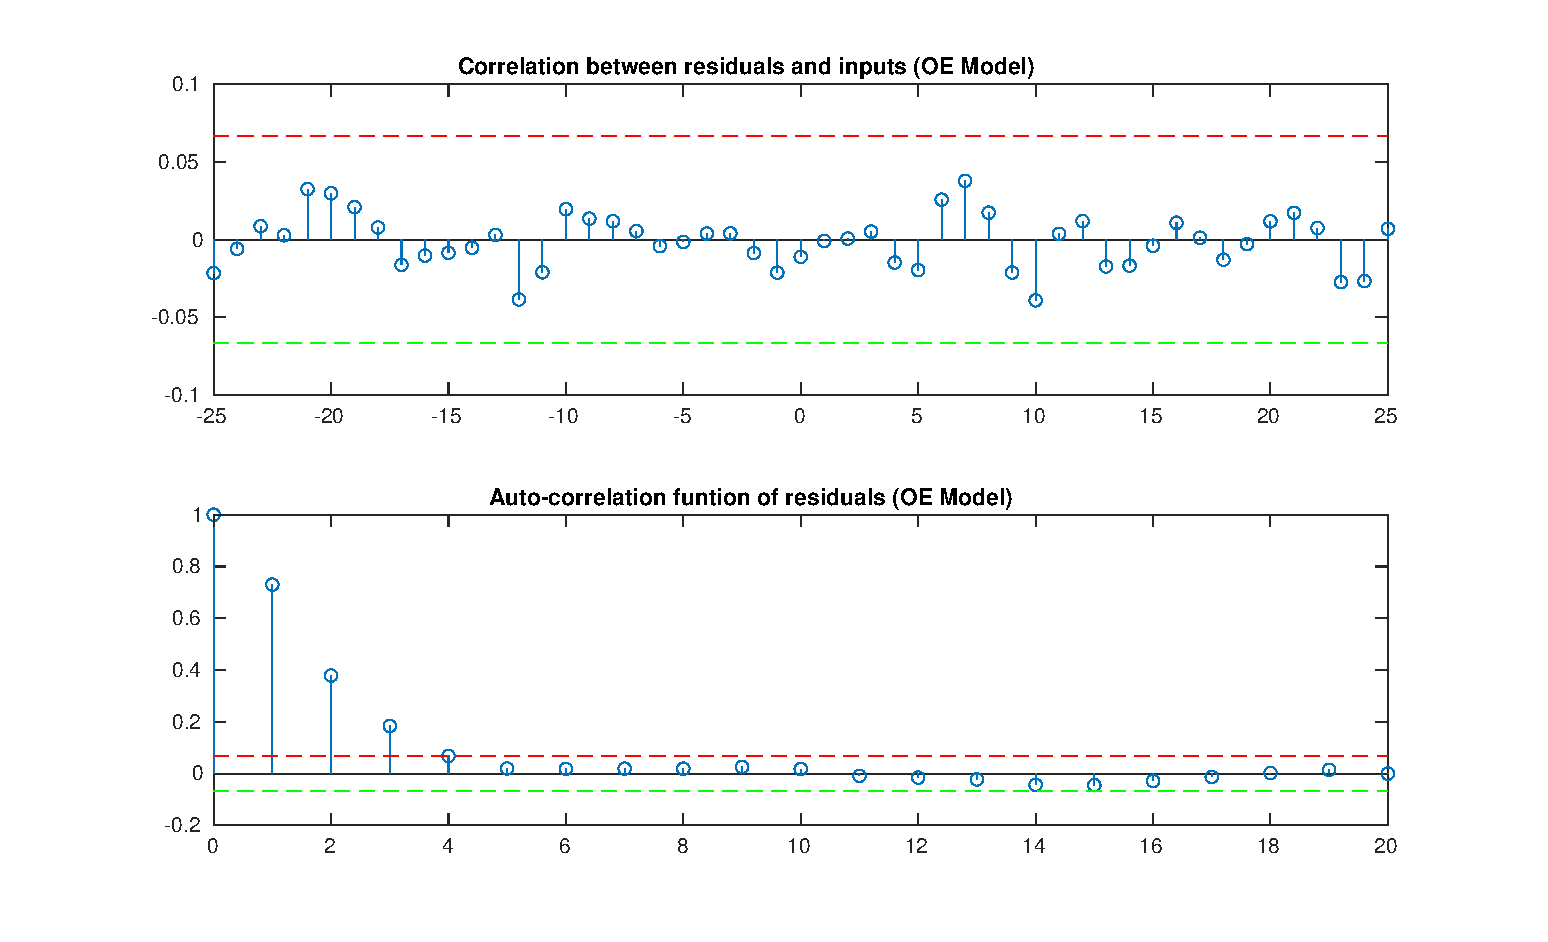
\includegraphics[width=\maxwidth{100.35122930255896em}]{figure_6.eps}
\end{center}


\vspace{1em}
\begin{par}
\begin{center}
BJ model:
\end{center}
\end{par}

\begin{matlabcode}
% BJ model:
mod_bj = bj(Ztrain ,[1 1 1 1 2]);
present(mod_bj)
\end{matlabcode}
\begin{matlaboutput}
                                                                              
mod_bj =                                                                      
Discrete-time BJ model: y(t) = [B(z)/F(z)]u(t) + [C(z)/D(z)]e(t)              
  B(z) = 2.005 (+/- 0.009254) z^-2                                            
                                                                              
  C(z) = 1 + 0.5922 (+/- 0.02454) z^-1                                        
                                                                              
  D(z) = 1 - 0.5185 (+/- 0.02609) z^-1                                        
                                                                              
  F(z) = 1 - 0.5151 (+/- 0.005275) z^-1                                       
                                                                              
Sample time: 1 seconds                                                        
                                                                              
Parameterization:                                                             
   Polynomial orders:   nb=1   nc=1   nd=1   nf=1   nk=2                      
   Number of free coefficients: 4                                             
   Use "polydata", "getpvec", "getcov" for parameters and their uncertainties.
                                                                              
Status:                                                                       
Termination condition: Near (local) minimum, (norm(g) < tol)..                
Number of iterations: 2, Number of function evaluations: 5                    
                                                                              
Estimated using BJ on time domain data "Ztrain".                              
Fit to estimation data: 84.88% (prediction focus)                             
FPE: 0.101, MSE: 0.1004                                                       
More information in model's "Report" property.                                
\end{matlaboutput}
\begin{matlabcode}
yhat_bj = predict(mod_bj, Ztrain );       % Predictions on training data
err_bj = pe(mod_bj, Ztrain );             % Compute one-step ahead prediction errors

% Residual analysis:
cross_corr_bj = xcov(err_bj.y, Ztrain.u,25,'coeff');
acf_bj = xcov(err_bj.y,20,'coeff');

% Plot
figure;set(gcf,'position',[10,10,1000,600]);

subplot(211); stem( -25:25 , cross_corr_bj ); hold on
plot([ -25 25] ,[1 1]* clim ,'r--' ,[-25 25] ,[ -1 -1]*clim ,'g--')
title('Correlation between residuals and inputs (BJ Model)')
ylim([-0.4 0.4])

subplot(212); stem((0:20) ,acf_bj (21:end)); hold on
plot([0 20] ,[1 1]* clim ,'r--' ,[0 20] ,[ -1 -1]*clim ,'g--')
title('Auto-correlation funtion of residuals (BJ Model)')
\end{matlabcode}
\begin{center}
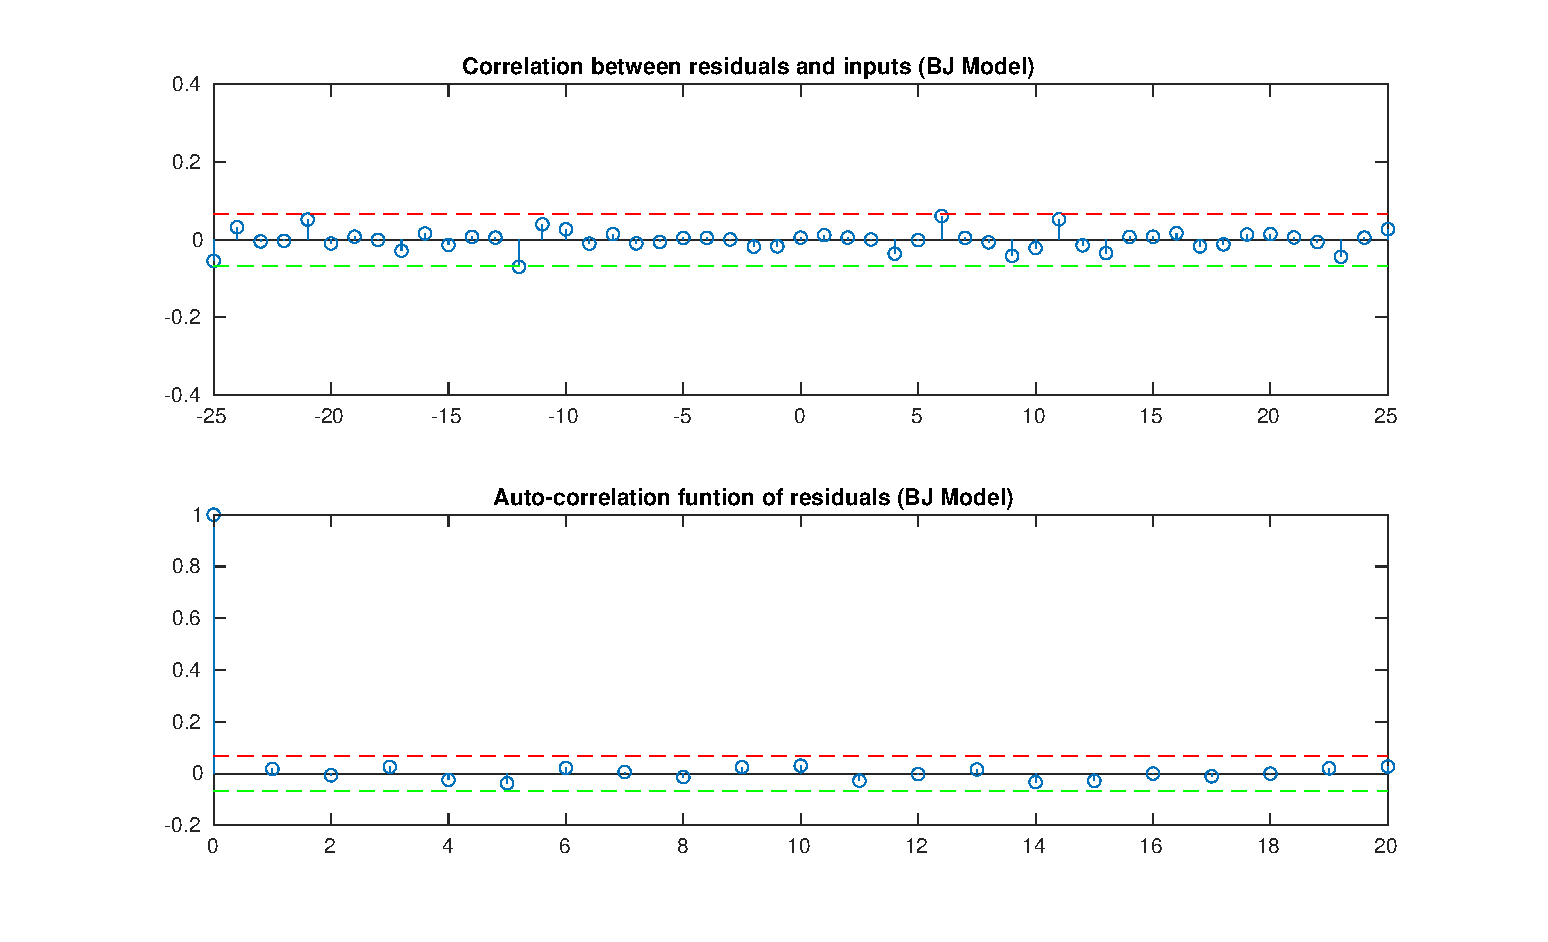
\includegraphics[width=\maxwidth{100.35122930255896em}]{figure_7.eps}
\end{center}
\begin{matlabcode}
% Predictions on test data
yhat_bj = predict(mod_bj, Ztest);

figure;set(gcf,'position',[10,10,1000,600]);
plot(linspace(1501,2045,545), Ztest.y, 'black'); hold on
plot(linspace(1501,2045,545), yhat_bj.y, 'r--');
legend('Original','Predicted');
\end{matlabcode}
\begin{center}
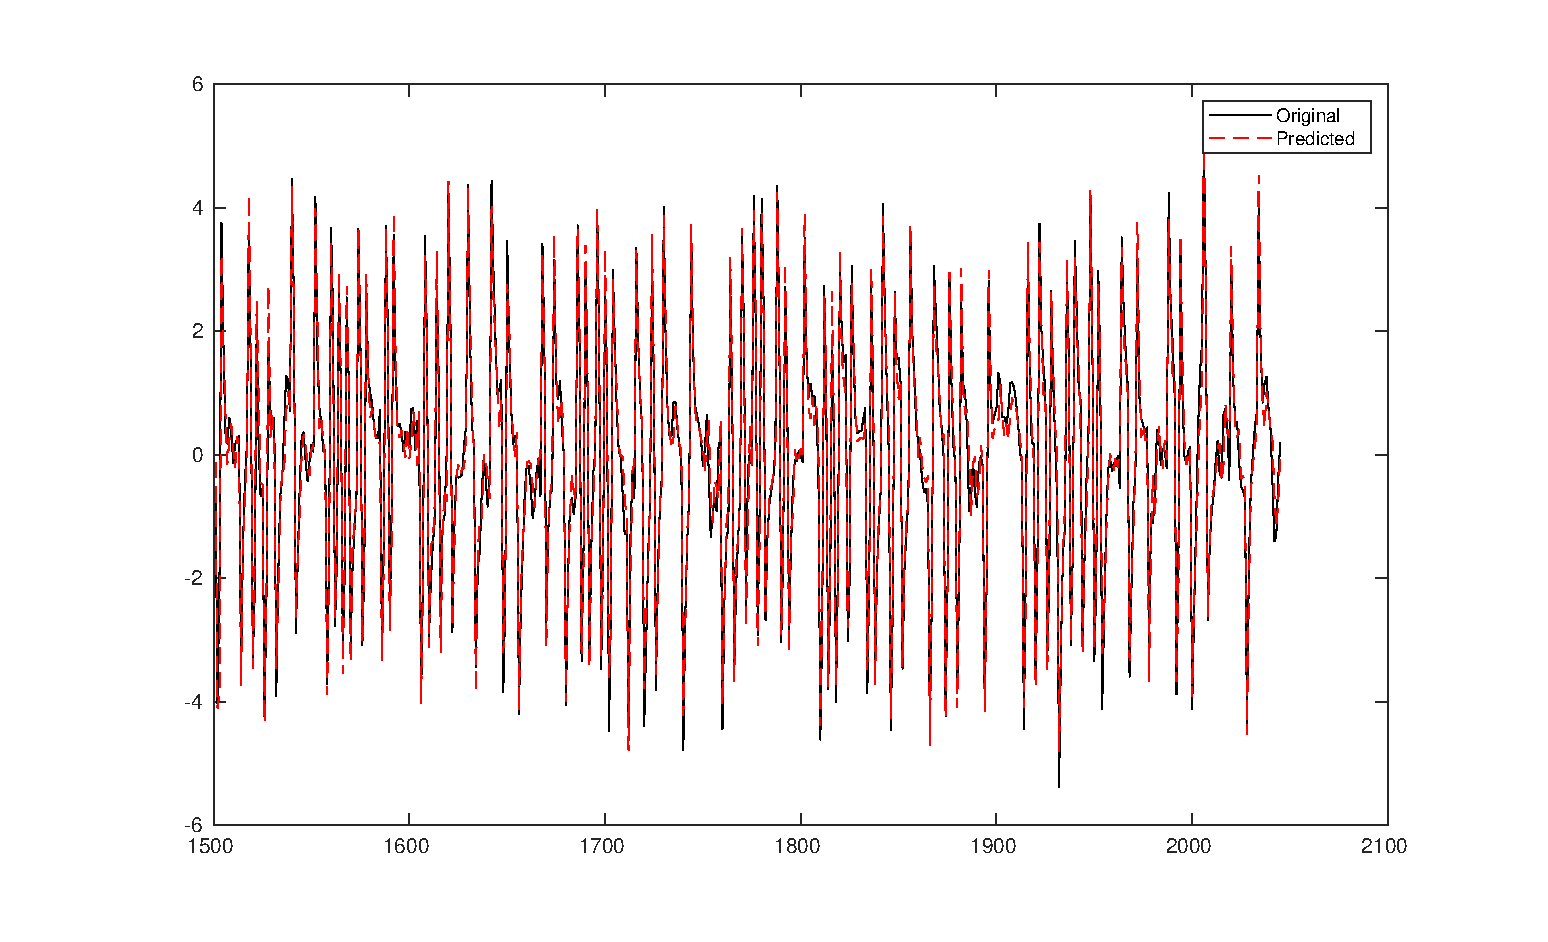
\includegraphics[width=\maxwidth{100.35122930255896em}]{figure_8.eps}
\end{center}


\vspace{1em}

\begin{par}
\begin{flushleft}
Question: 4.b)
\end{flushleft}
\end{par}

\begin{par}
\begin{center}
Without removing integrating effects:
\end{center}
\end{par}

\begin{matlabcode}
% Train-Test split:
dataset = iddata(iodata.yk, iodata.uk, 1);
datatrain = dataset (1:1500); datatest = dataset (1501:end);
[Ztrain ,Tr] = detrend(datatrain, 0);
Ztest = detrend(datatest, Tr);

% 99 % significance levels
clim = 2.58/sqrt(length(Ztrain.y));
\end{matlabcode}


\vspace{1em}
\begin{par}
\begin{center}
OE model: (white-noise assumption)
\end{center}
\end{par}

\begin{matlabcode}
% OE model:
mod_oe = oe(Ztrain ,[1 1 2]);
present(mod_oe);
\end{matlabcode}
\begin{matlaboutput}
                                                                              
mod_oe =                                                                      
Discrete-time OE model: y(t) = [B(z)/F(z)]u(t) + e(t)                         
  B(z) = 1.916 (+/- 0.08544) z^-2                                             
                                                                              
  F(z) = 1 - 0.4645 (+/- 0.0607) z^-1                                         
                                                                              
Sample time: 1 seconds                                                        
                                                                              
Parameterization:                                                             
   Polynomial orders:   nb=1   nf=1   nk=2                                    
   Number of free coefficients: 2                                             
   Use "polydata", "getpvec", "getcov" for parameters and their uncertainties.
                                                                              
Status:                                                                       
Termination condition: Near (local) minimum, (norm(g) < tol)..                
Number of iterations: 3, Number of function evaluations: 7                    
                                                                              
Estimated using OE on time domain data "Ztrain".                              
Fit to estimation data: 8.234%                                                
FPE: 35.67, MSE: 35.58                                                        
More information in model's "Report" property.                                
\end{matlaboutput}
\begin{matlabcode}
yhat_oe = predict(mod_oe , Ztrain );       % Predictions on training data
err_oe = pe(mod_oe , Ztrain );             % Compute one-step ahead prediction errors

% Residual analysis:
cross_corr_oe = xcov(err_oe.y, Ztrain.u,25,'coeff');
acf_oe = xcov(err_oe.y,20,'coeff');

% Plot
figure;set(gcf,'position',[10,10,1000,600]);

subplot(211); stem( -25:25 , cross_corr_oe ); hold on
plot([ -25 25] ,[1 1]* clim ,'r--' ,[-25 25] ,[ -1 -1]*clim ,'g--')
title('Correlation between residuals and inputs (OE Model)')
ylim([-0.4 0.4])

subplot(212); stem((0:20) ,acf_oe (21:end)); hold on
plot([0 20] ,[1 1]* clim ,'r--' ,[0 20] ,[ -1 -1]*clim ,'g--')
title('Auto-correlation funtion of residuals (OE Model)')
\end{matlabcode}
\begin{center}
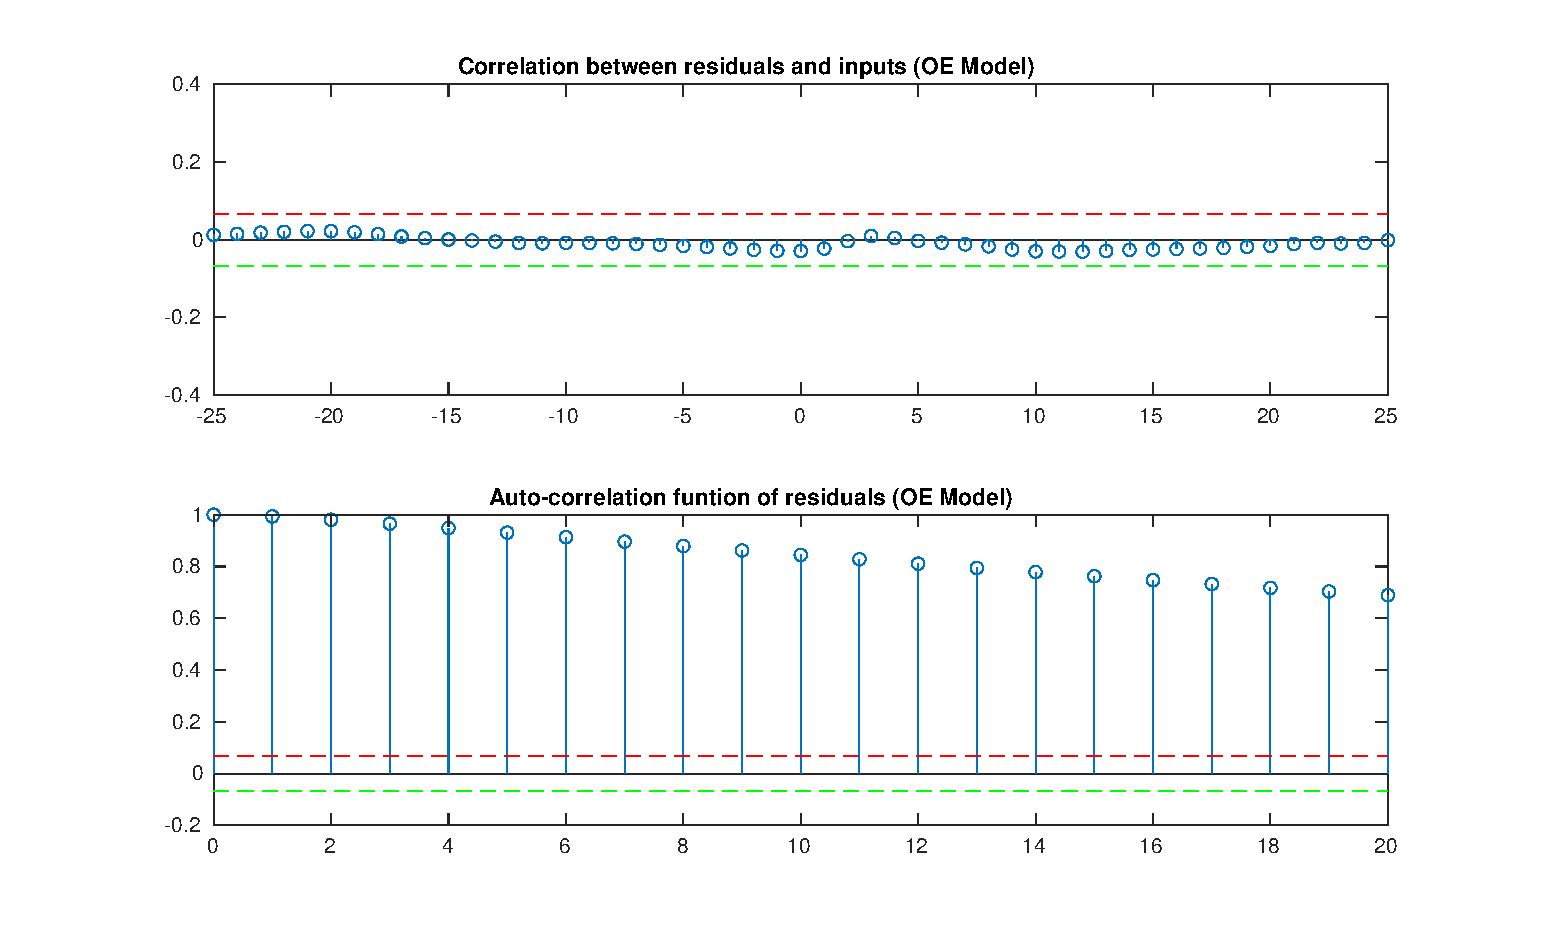
\includegraphics[width=\maxwidth{100.35122930255896em}]{figure_9.eps}
\end{center}


\vspace{1em}
\begin{par}
\begin{center}
BJ model:
\end{center}
\end{par}

\begin{matlabcode}
% BJ model:
% [1 3 3 1 2] --> [1 1 2 1 2]
mod_bj = bj(Ztrain ,[1 1 2 1 2]);
present(mod_bj)
\end{matlabcode}
\begin{matlaboutput}
                                                                              
mod_bj =                                                                      
Discrete-time BJ model: y(t) = [B(z)/F(z)]u(t) + [C(z)/D(z)]e(t)              
  B(z) = 2.005 (+/- 0.009104) z^-2                                            
                                                                              
  C(z) = 1 + 0.6155 (+/- 0.02354) z^-1                                        
                                                                              
  D(z) = 1 - 1.507 (+/- 0.02476) z^-1 + 0.5134 (+/- 0.02482) z^-2             
                                                                              
  F(z) = 1 - 0.5147 (+/- 0.005215) z^-1                                       
                                                                              
Sample time: 1 seconds                                                        
                                                                              
Parameterization:                                                             
   Polynomial orders:   nb=1   nc=1   nd=2   nf=1   nk=2                      
   Number of free coefficients: 5                                             
   Use "polydata", "getpvec", "getcov" for parameters and their uncertainties.
                                                                              
Status:                                                                       
Termination condition: Near (local) minimum, (norm(g) < tol)..                
Number of iterations: 4, Number of function evaluations: 9                    
                                                                              
Estimated using BJ on time domain data "Ztrain".                              
Fit to estimation data: 95.26% (prediction focus)                             
FPE: 0.09611, MSE: 0.09509                                                    
More information in model's "Report" property.                                
\end{matlaboutput}
\begin{matlabcode}
yhat_bj = predict(mod_bj, Ztrain );       % Predictions on training data
err_bj = pe(mod_bj, Ztrain );             % Compute one-step ahead prediction errors

% Residual analysis:
cross_corr_bj = xcov(err_bj.y, Ztrain.u,25,'coeff');
acf_bj = xcov(err_bj.y,20,'coeff');

% Plot
figure;set(gcf,'position',[10,10,1000,600]);

subplot(211); stem( -25:25 , cross_corr_bj ); hold on
plot([ -25 25] ,[1 1]* clim ,'r--' ,[-25 25] ,[ -1 -1]*clim ,'g--')
title('Correlation between residuals and inputs (BJ Model)')
ylim([-0.4 0.4])

subplot(212); stem((0:20) ,acf_bj (21:end)); hold on
plot([0 20] ,[1 1]* clim ,'r--' ,[0 20] ,[ -1 -1]*clim ,'g--')
title('Auto-correlation funtion of residuals (BJ Model)') 
\end{matlabcode}
\begin{center}
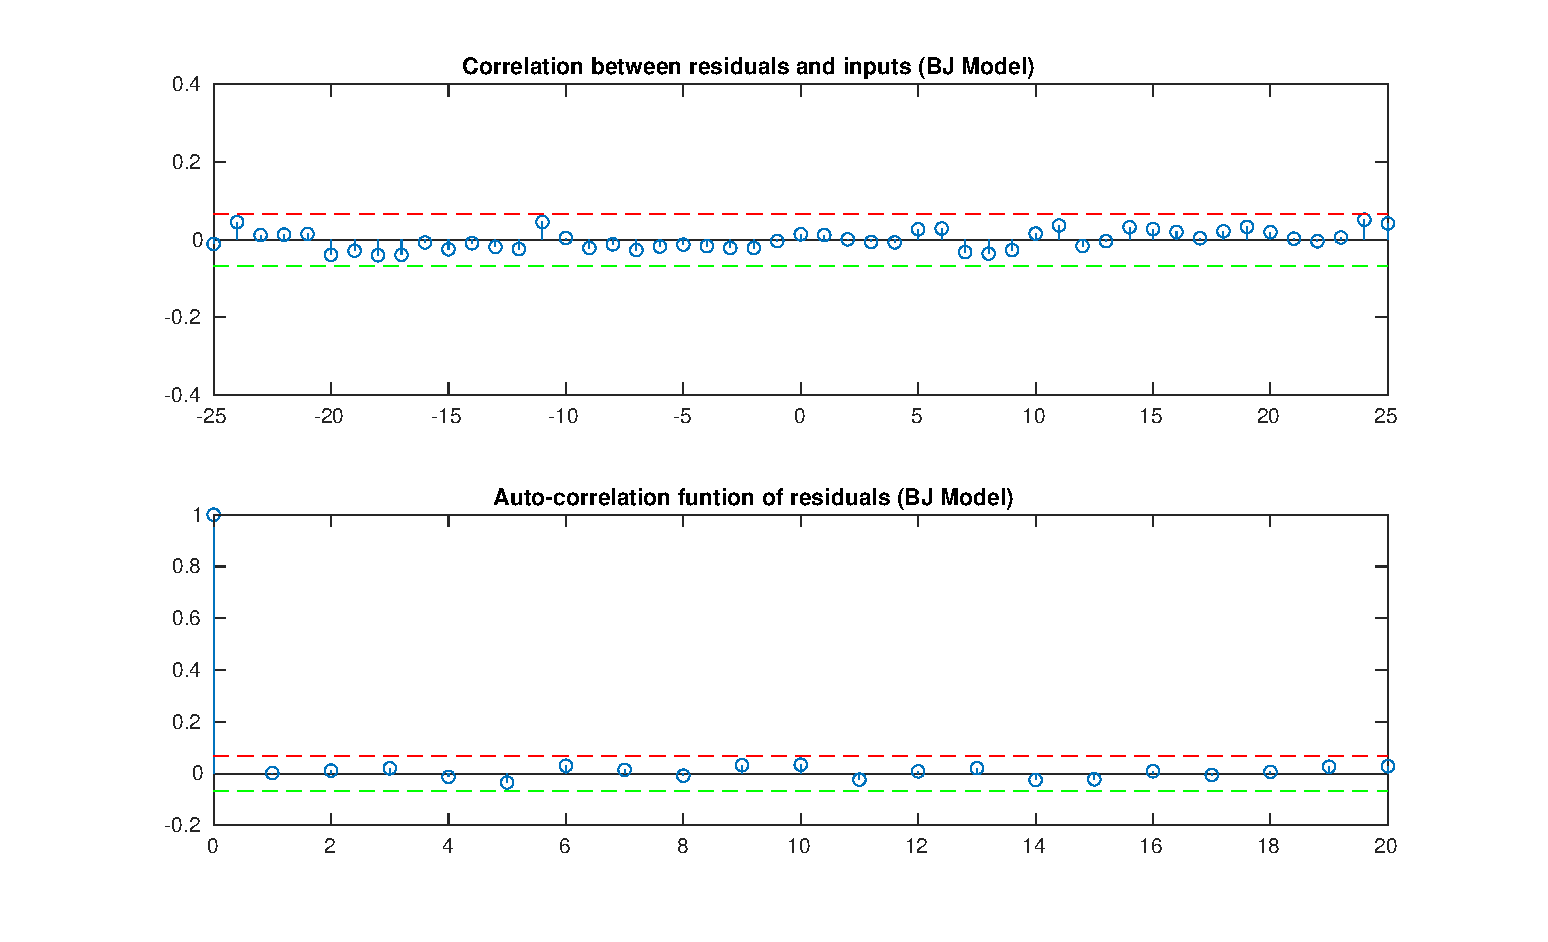
\includegraphics[width=\maxwidth{100.35122930255896em}]{figure_10.eps}
\end{center}


\begin{matlabcode}
% Predictions on test data
yhat_bj = predict(mod_bj, Ztest);

figure;set(gcf,'position',[10,10,1000,600]);
plot(linspace(1501,2046,546), Ztest.y, 'black'); hold on
plot(linspace(1501,2046,546), yhat_bj.y, 'r--');
legend('Original','Predicted');
\end{matlabcode}
\begin{center}
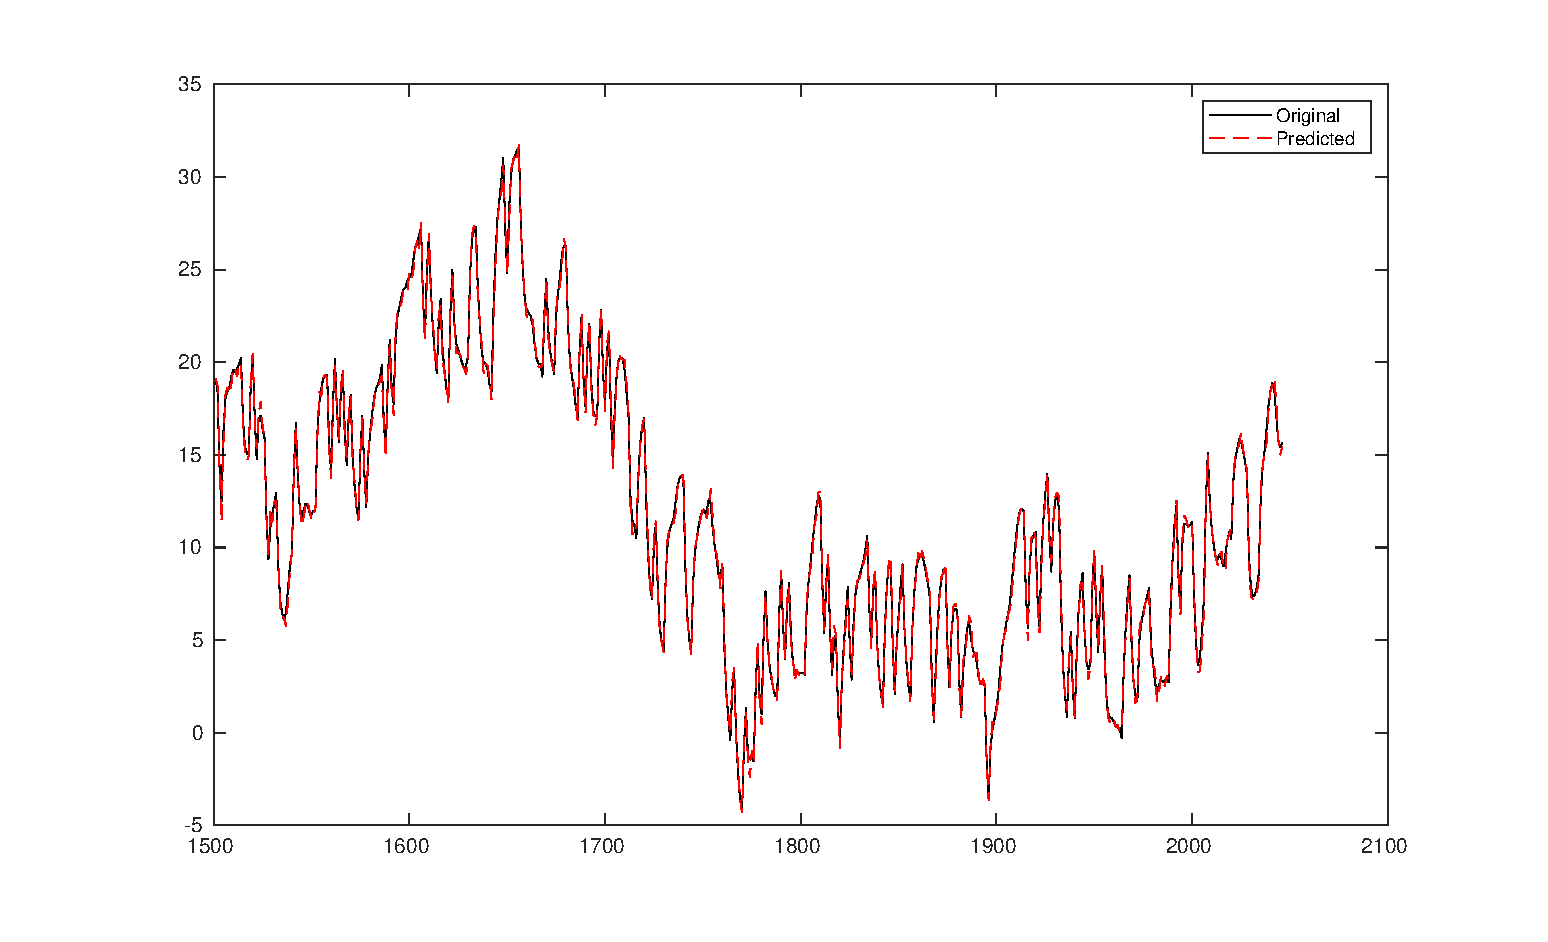
\includegraphics[width=\maxwidth{100.35122930255896em}]{figure_11.eps}
\end{center}
\begin{matlabcode}

\end{matlabcode}


\begin{par}
\begin{flushleft}
Question: 5.a)
\end{flushleft}
\end{par}

\begin{matlabcode}
% Increase precision of double to 200 (whichever is enclosed by vpa() function)
d1 = digits(200);

N = 100;
mod_p = idpoly(1, [0 2 1.4], 1, 1, 1,'Noisevariance', 1,'Ts',1);
uk = idinput(N+2,'PRBS', [0 1], [-1 1]);

% Calculate yk_star:
yk_star = sim(mod_p ,uk);
mod_p.Noisevariance = var(yk_star) / 10;

% Calculate yk:
yk = sim(mod_p ,uk , simOptions ('AddNoise',true));


syms y mu stdev
pdf_guassian = ((1/sqrt(2*pi*stdev.^2))*exp(-(((y-mu)/stdev).^2)/2));

syms b1 b2 mu1 mu2 stdev1 stdev2
joint_gaussian_pdf = ((1/sqrt(2*pi*stdev1.^2))*exp(-(((b1-mu1)/stdev1).^2)/2)).*((1/sqrt(2*pi*stdev2.^2)).*exp(-(((b2-mu2)/stdev2).^2)/2));

likelihood = 1;
for k = 3:N+2
    pdf_yk = subs(pdf_guassian, {y,mu,stdev},  {yk(k), b1*uk(k-1) + b2*uk(k-2), sqrt(var(yk))});
    likelihood = likelihood .* pdf_yk;
end


prior = subs(joint_gaussian_pdf, {mu1, mu2, stdev1, stdev2}, {0, 0, 5, 5})
\end{matlabcode}
\begin{matlabsymbolicoutput}
prior = 

\hskip1em $\displaystyle \frac{{\mathrm{e}}^{-\frac{{b_1 }^2 }{50}} \,{\mathrm{e}}^{-\frac{{b_2 }^2 }{50}} }{50\,\pi }$
\end{matlabsymbolicoutput}
\begin{matlabcode}
f_yn = vpa(integral2(matlabFunction(likelihood .* prior), -Inf, Inf, -Inf, Inf));
posterior = (1/f_yn) * vpa(likelihood * prior);

mom_1 = matlabFunction(b1 .* posterior);
mom_2 = matlabFunction(b1^2 .* posterior);

integral2(mom_1, -Inf, Inf, -Inf, Inf)
\end{matlabcode}
\begin{matlaboutput}
ans = 1.9969
\end{matlaboutput}
\begin{matlabcode}

mom_1 = matlabFunction(b2 .* posterior);
integral2(mom_1, -Inf, Inf, -Inf, Inf)
\end{matlabcode}
\begin{matlaboutput}
ans = 1.3989
\end{matlaboutput}
\begin{matlabcode}

\end{matlabcode}

\end{document}
